\chapter{Quantum annealing and GPU computing}
\label{chapter:near-term}

After introducing the Ising model, our next task is to present the technologies
used in the research conducted for this thesis. Since the main point of this
thesis is benchmarking quantum annealers, it is only natural that we start by
introducing the reader to the concepts of adiabatic quantum computations and
quantum annealing. The second part of the chapter is devoted to Nvidia CUDA, a
technology allowing massively parallel computations on general-purpose graphics
processing units (GPUs).

\section{Adiabatic quantum computation and quantum annealing}
\sectionmark{AQC and quantum annealing}

\subsection{Adiabatic Quantum Computation}
One of the possible models of quantum computing is Adiabatic Quantum
Computation (AQC) \cite{farhi}. AQC ties closely with quantum annealing, and
hence we will shortly discuss how it works in general. Before we describe how
the computations are performed in this model, we will take a closer look at the
underlying adiabatic theorem, which can be stated as follows \cite{farhi,
  born}:

\begin{theorem}[Adiabatic theorem]
  Suppose we are give a time-dependent Hamiltonian $\tilde{H}(t)$ with
  eigenenergies $E_1(t) \le E_2(t) \le \ldots \le E_i(t) \le \ldots$ and
  corresponding eigenstates $\ket{\psi_i(t)}$. Further, suppose we are given a
  physical system $\mathcal{S}$ evolving according to $H(t) = \tilde{H}(t/T)$ and
  let $\ket{\psi(t)}$ denote the state of $\mathcal{S}$ at time $t$. If
  $\ket{\psi(0)} = \ket{\psi_n(0)}$, then also $\ket{\psi(t)} = \ket{\psi_n(t)}$
  for all time $t$, provided that $T$ is large enough and for all $t$ there
  exists a non-zero difference between $E_n(t)$ and the rest of the $H(t)$'s
  spectrum.
\end{theorem}

One conclusion to the adiabatic theorem is of particular importance to quantum
computation. If the system is prepared in a ground state, has a non-zero gap
between its ground energy and the energy of the first excited state, and is
evolved slowly enough, it will stay in the ground state during the whole
evolution. Knowing this we can finally discuss how AQC works. First, an
optimization problem to be solved is encoded as a ground state of some
Hamiltonian $\HH_{target}$. Then, a physical system is prepared in a ground state
of some simpler Hamiltonian, $\HH_{initial}$. After that, the system is driven
slowly from $\HH_{initial}$ to $\HH_{target}$. By adiabatic theorem, the system
ends up in a ground state of $\HH_{target}$, and after the measurement is
performed the solution to the original problem can be decoded.

In Quantum Annealing (QA), one follows essentially the same procedure as in
Adiabatic Quantum Computing. What is different, is that the evolution of the
system in QA does not have to be adiabatic \cite{Vinci2017}. We will describe
in more detail how Quantum Annealing works on a concrete example later in this
chapter when we discuss D-Wave annealers.

\subsection{D-Wave quantum annealers}

The first commercially available quantum annealer was D-Wave One, which was
introduced by D-Wave company in $2011$ \cite{johnson}, featuring 128 qubits.
Since then, multiple improved generations of D-Wave annealers have been
released. At the time of writing, the newest series of D-Wave annealers is
called the Advantage system. Devices in this series utilize a chip with at
least $5000$ qubits. Table \ref{tab:dwave} summarizes the release history of
D-Wave annealers and highlights the differences between their generations.

As already mentioned in the introduction, D-Wave annealers are built to find
the ground states of the classical Ising spin--glasses. In these devices, the
spin variables correspond to physical two-level systems, called qubits. At the
end of the annealing process, the (quantum) Hamiltonian of the annealer has to
correspond to the classical Ising Hamiltonian of the spin--glass instance being
solved, i.e.:
\begin{equation}
  \HH_{target} = \sum_{i=1}^N h_i \ssigma^{(i)}_z + \sum_{<i, j>} J_{ij} \ssigma^{(i)}_z \ssigma^{(j)}_z,
\end{equation}
where $N$, as previously, is the number of spins, $\ssigma^{(i)}_x$,
$\ssigma^{(i)}_z$ denote Pauli operators acting on $i$-th qubit, and $h_i,
  J_{ij} \in \mathbb{R}$ are coefficients of the instance. More precisely, the
time-dependent Hamiltonian implemented by the D-Wave devices is of the form:
\begin{equation}
  \label{eq:dwaveham}
  \HH(t) =  -\frac{A(t)}{2}\sum_{i=1}^N \ssigma^{(i)}_x + \frac{B(t)}{2}\left(\sum_{i=1}^N h_i \ssigma^{(i)}_z + \sum_{<i, j>} J_{ij} \ssigma^{(i)}_z \ssigma^{(j)}_z\right).
\end{equation}
where $t \in [0, \tau]$ \cite{dwavedocs}. The tunneling energy curve $A(t)$ is
monotonically decreasing and it vanishes as $t$ approaches $\tau$. Similarly
$B(t)$ is monotonically increasing, and the functions satisfy $A(0) \gg B(0)$
and $B(\tau) \gg A(\tau)$.

Since the variables in the spin--glass being solved have to correspond to the
physical qubits, it is clear that the number of qubits of the device limits the
size of the input problem. However, it is not the only factor restricting
problems that can be directly submitted to the annealer. To implement quadratic
terms in the Ising hamiltonian, the qubits have to be physically connected via
a \emph{coupler}. The available connectivity on the device depends on two
factors. The first one is the \emph{topology} of the chip, i.e. graph
describing its qubits layout. The topology is the same for all devices in the
same generation. However, due to manufacturing errors and calibration problems,
some qubits and/or couplers might be unavailable to the end user. The graph
describing qubits' connectivity of an actual device is called its \emph{working
  graph}. Understanding annealer topologies is crucial for understanding how to
program these devices. Hence, in the next section, we will describe topologies
of all currently available D-Wave annealers

\begin{table}
  \footnotesize
  \centering

  \begin{tabular}[pos]{|>{\columncolor{tsubheader}}l|c|c|c|c|}
    \hline
    \rowcolor{theader}
    \textbf{Series}       &
    \textbf{Release year} &
    \textbf{Topology}     &
    \textbf{Num. qubits}  &
    \textbf{Num. couplers}                                      \\
    \hline
    D-Wave One            & 2011      & $C_{4}$  & 128  & 352   \\
    \hline
    D-Wave Two            & 2013      & $C_{8}$  & 512  & 1472  \\
    \hline
    D-Wave 2X             & 2015      & $C_{12}$ & 1152 & 3360  \\
    \hline
    D-Wave 2000Q          & 2017      & $C_{16}$ & 2048 & 6016  \\
    \hline
    Advantage             & 2020      & $P_{16}$ & 5640 & 40484 \\
    \hline
    Advantage 2           & 2023-2024 & $Z_{15}$ & 7440 & 71736 \\
    \hline
  \end{tabular}
  \caption{
    Comparison of different generations of D-Wave annealers. For topologies, $C_n$,
    $P_n$ and $Z_n$ refers to Chimera, Pegasus and Zephyr of size $n$ respectively.
    The numbers of qubits and couplers are given for a perfectly manufactured chip
    with full yield. Actual devices from any series typically have a lower number
    of qubits and/or couplers.}. \label{tab:dwave}
\end{table}

% \begin{figure}
%     \centering
%     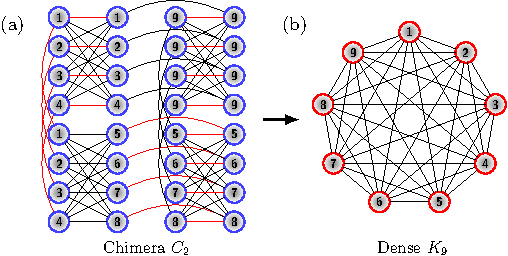
\includegraphics[width=\textwidth]{figures/chimera.pdf}
%     \caption{\textbf{a.} Example of Chimera topology. Graph presented here consists of a $2 \times 2$ grid of unit cells (hence $C_2$ the name). Note the sparse connectivity of the presented graph as compared to the full graph with the same number of nodes. \textbf{b.} Full $K_9$ graph embedded in Chimera graph from \textbf{a.}. The nodes are labelled with numbers corresponding to groups of logical qubits they were constructed from.}
%     \label{fig:chimera}
% \end{figure}

\subsection{Annealer topologies}

The first topology that we will discuss in this chapter is the \emph{Chimera}
topology, used for all generations of D-Wave devices up to D-Wave 2000Q series.
We decided to describe the Chimera before moving towards newer topologies
because it serves as a building block for its successors.

While discussing the topologies of the D-Wave annealers, we will not discuss
the physical structure of the chip. We decided to do so because, for this
thesis, the \emph{logical} structure of the chip is far more important than the
underlying physical one. However, one consequence of this choice is that the
distinction between two types of couplers (external and internal) will become
less intuitive once we reach beyond the Chimera topology. Nevertheless, we
believe that this will not impair the reader's ability to understand the layout
of qubits in the newer devices. For the description of the physical chip
layouts, we refer the reader to \cite{dwavedocs}.

\subsubsection{The Chimera topology}

In Chimera topology, depicted in Fig. \ref{fig:chimera}, the qubits are placed
on a rectangular grid of \emph{unit cells}. Every unit cell is a complete
bipartite graph $K_{t,t}$. Each group in the bipartition is called
\emph{shore}, and hence the parameter $t$ is called the \emph{shore size}. Each
qubit in the unit cell (except the ones in the cells on the border) connects to
two qubits on the same shore in the neighboring cells. Hence, the whole Chimera
graph is also bipartite, and the maximum degree of a node is $t+2$. The
couplers connecting qubits in the same unit cell are called \emph{internal} and
the couplers connecting qubits belonging to different cells are called
\emph{external}.

Typically, the devices using Chimera topology utilize a square grid with a
shore size of $4$. Such layouts are denoted by $C_n$, where $n$ is the width
(and the height) of the grid. In such devices, each qubit is connected to a
maximum of 6 qubits, the total number of qubits is $8n^2$ and the total number
of couplers is $16n^2 + 8(n-1)n$.

The Chimera topology is often visualized using two distinct layouts, both of
which are exemplified in Fig. \ref{fig:chimera}. In the cross layout, the
shores of the unit cell form a cross, with one shore being placed vertically
and the second shore being placed horizontally. In the grid layout, each unit
cell is depicted as two columns of qubits, corresponding to both shores of the
cell. While the grid layout might be more intuitive in some applications, cross
layouts are in turn convenient when presenting the Pegasus topology, which we
will discuss next.

\begin{figure}
  \begin{subfigure}[b]{0.5\textwidth}
    \centering
    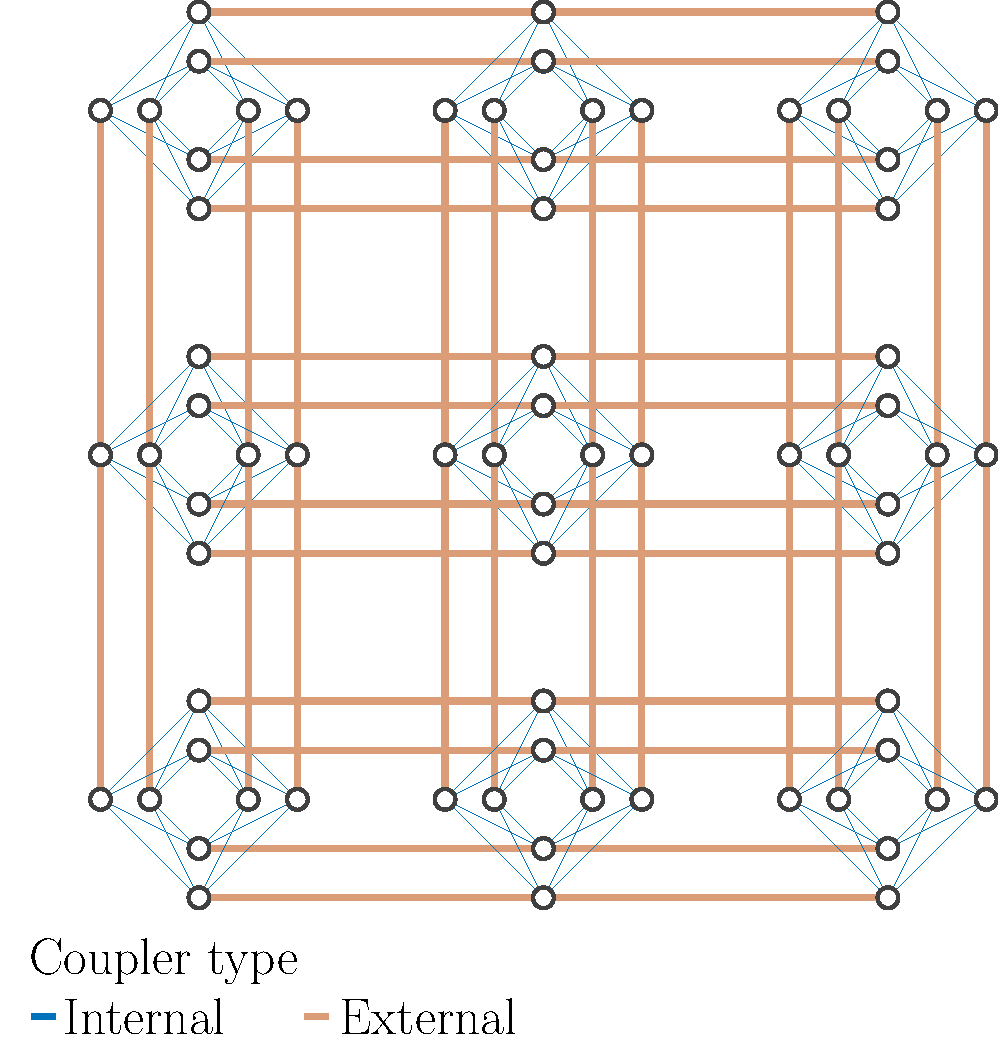
\includegraphics[width=0.8\textwidth]{figures/chimera-cross.pdf}
    \caption{}\label{fig:chimera-cross}
  \end{subfigure}
  \begin{subfigure}[b]{0.45\textwidth}
    \centering
    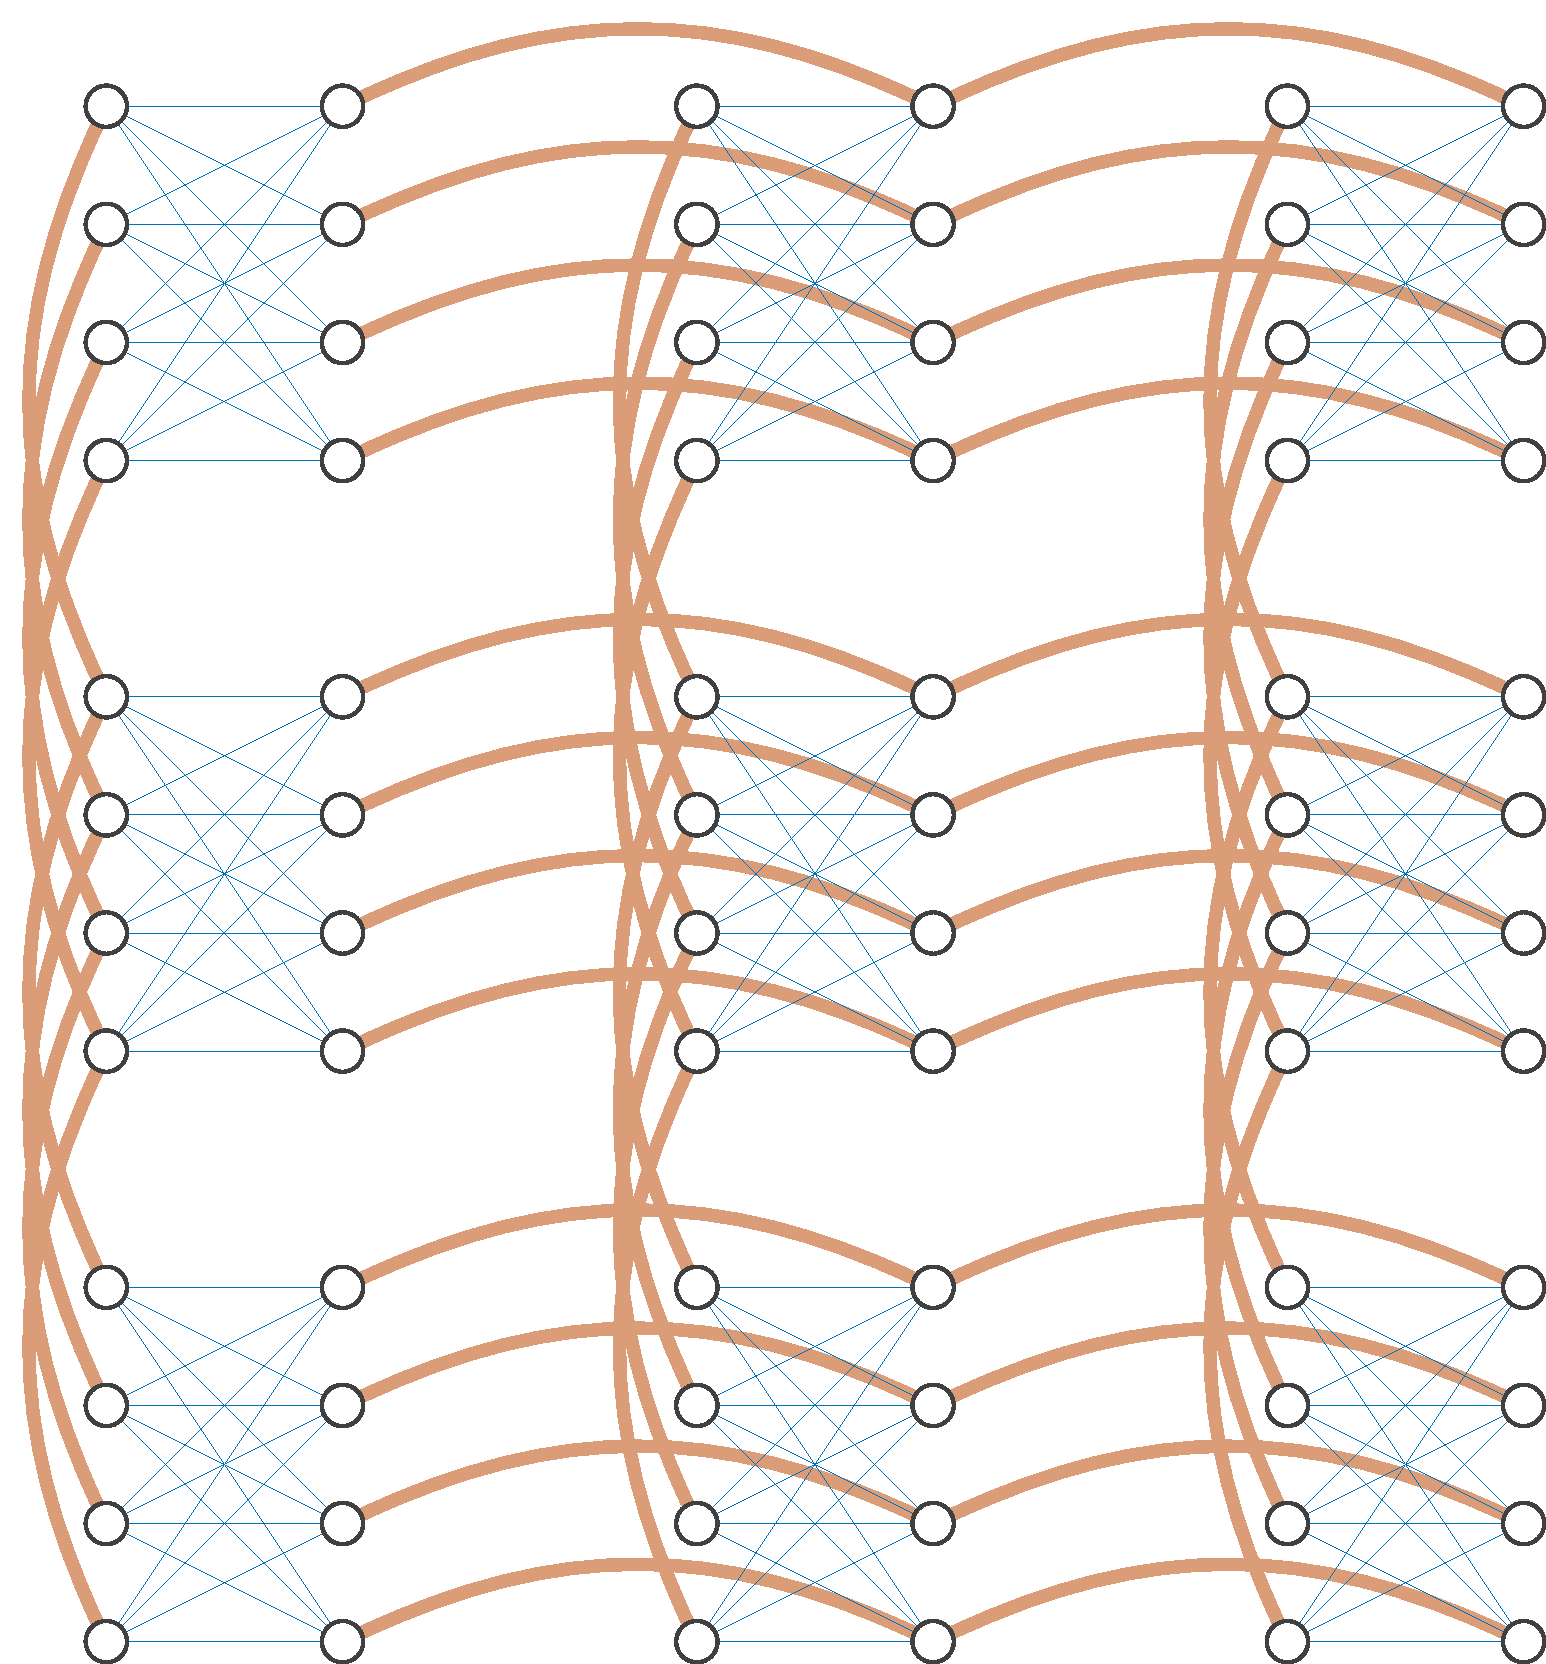
\includegraphics[width=0.8\textwidth]{figures/chimera-shore-column.pdf}
    \caption{}\label{fig:chimera-shore-column}
  \end{subfigure}
  \caption{
    Chimera $C_3$ topology drawn using different layouts.
    \subref{fig:chimera-cross} The cross layout. \subref{fig:chimera-shore-column}
    The grid layout. The internal couplers are marked with {\color{RoyalBlue} blue},
    and the external couplers are marked with {\color{Tan} orange}. }
  \label{fig:chimera}
\end{figure}

\subsubsection{The Pegasus topology}
The current generation of D-Wave devices, dubbed the Advantage System, uses a
topology called Pegasus \cite{boothby}. An example of this topology is
presented in Fig. \ref{fig:pegasus}. The unit cell of Pegasus comprises 24
qubits grouped into the 3 Chimera unit cells. The topology features several
improvements regarding the qubit connectivity. Firstly, the internal couplers
connect not only the qubits in the same Chimera unit cell but also connect some
neighboring Chimera unit cells. Secondly, inside the Chimera unit cells new
type of connection, called \emph{the odd} couplers, is introduced.
Interestingly, those modifications mean that the Pegasus graph is no longer
bipartite. The Pegasus topology having $n$ rows and $n$ columns of unit cells
is denoted by $P_n$ and contains $24n(n-1)$ qubits.

Observe that a graph in Pegasus topology features subgraphs isomorphic to
Chimera graphs. This fact is important for the annealer users, as all problems
instances compatible with a device using the Chimera topology are automatically
compatible with annealers using a sufficiently large Pegasus topology.

\begin{figure}
  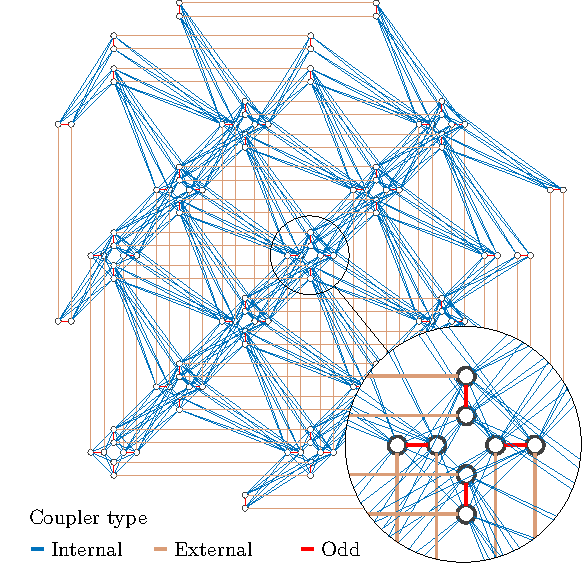
\includegraphics[width=\textwidth]{figures/pegasus}
  \caption{
    The $P_3$ graph, an example of the Pegasus topology. The magnified portion of
    the image shows a part of the graph containing a Chimera unit cell. Observe the
    odd couplers, marked in red, connecting qubits that are not connected in a unit
    cell of Chimera topology. } \label{fig:pegasus}
\end{figure}

\subsection{The Zephyr topology}
The upcoming generation of D-Wave annealers, called Advantage 2 System, will
use the Zephyr topology \cite{zephyr}. This topology utilizes Chimera unit
cells with a shore size of 8 and, compared to the Pegasus topology, contains
more odd couplers. Overall, the maximum degree of a qubit in Zephyr topology is
20. The Zephyr topology containing $n$ unit cells is denoted $Z_n$ and contains
$16n(2n+1)$ qubits.

\begin{figure}
  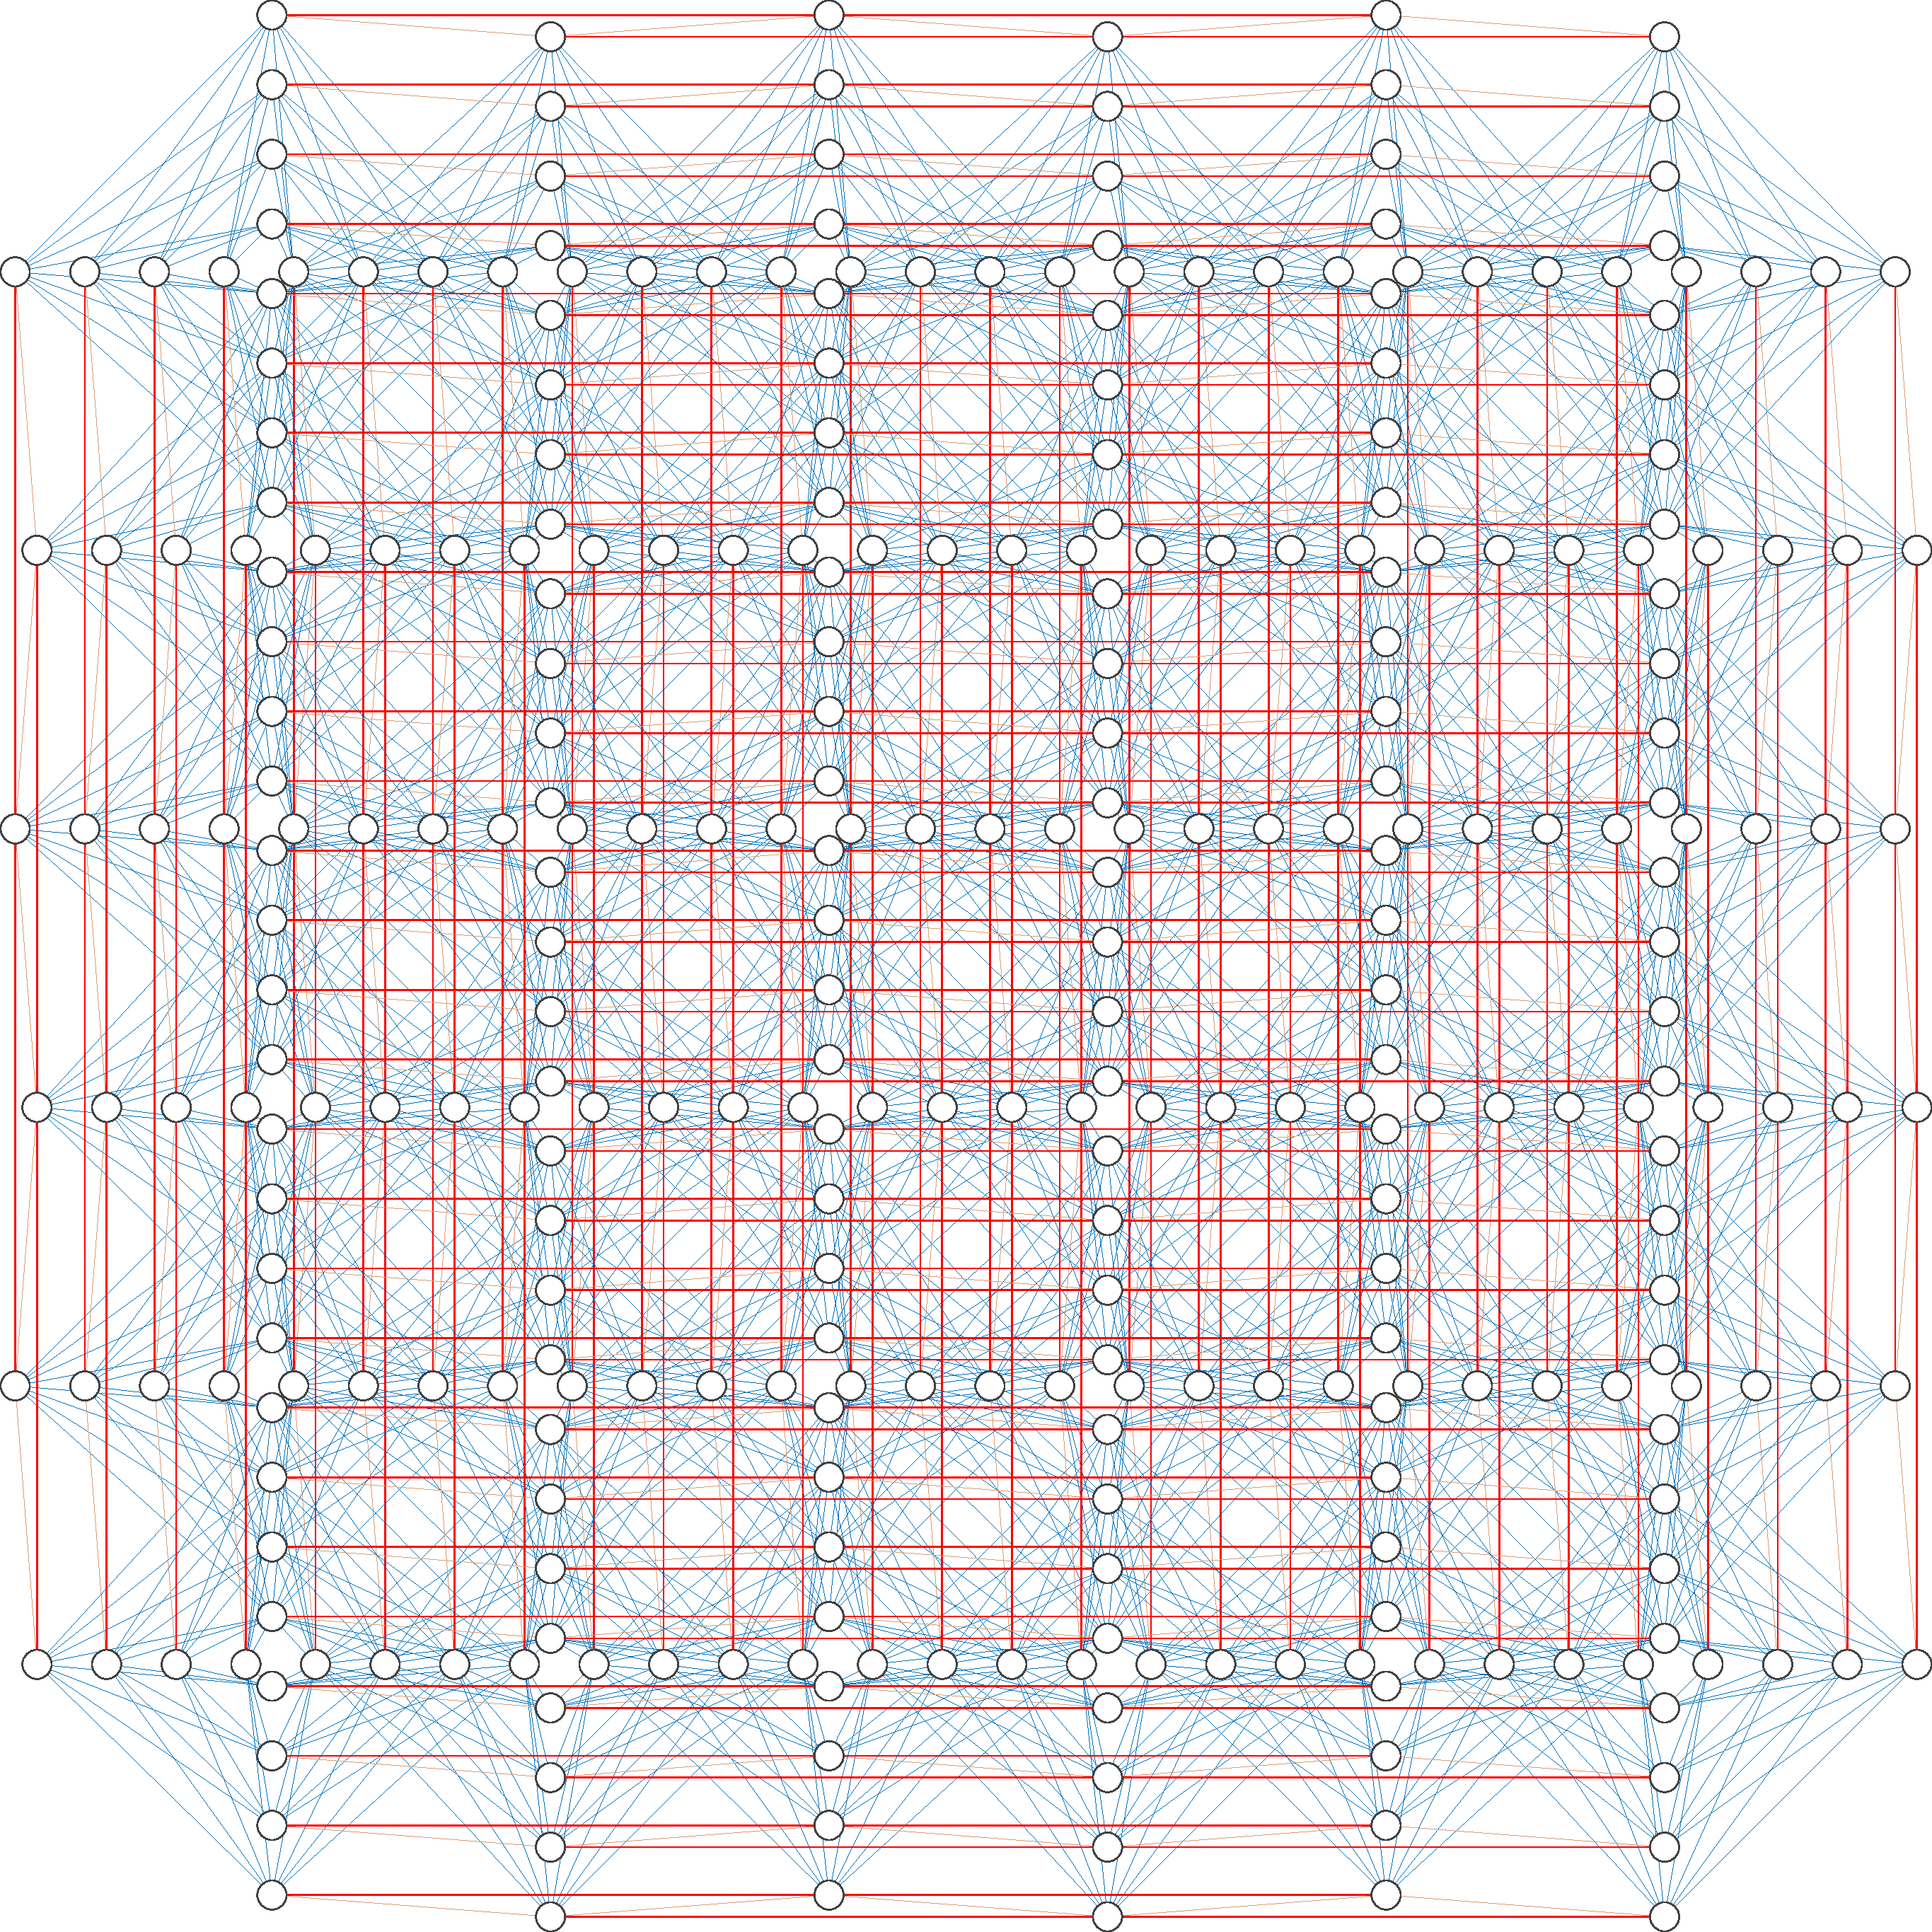
\includegraphics[width=\textwidth]{figures/zephyr}
  \caption{
    The $Z_3$ graph, an example of the Zephyr topology. Different types of couplers
    are color--coded. Observe that, similarly to Pegasus, the Zephyr topology
    contains Chimera subgraphs. However, the shore size of the Chimera unit cells
    in Zephyr is 8 instead of 4. } \label{fig:zephyr}
\end{figure}

\subsection{Minor embeddings}

Oftentimes, even small (relatively to the available number of qubits) instances
are not compatible with the annealer because of its restricted connectivity.
This issue can sometimes be mitigated using a procedure called the \emph{minor
  embedding}, in which the number of qubits is sacrificed for an improvement in
connectivity. Informally, the minor embedding relies on constructing a new
\emph{logical} graph with which the Ising instance to be solved is compatible.
This, in turn, is achieved by introducing \emph{logical} qubits built from
several physical qubits (a process called \emph{contraction}). For the reasons
explained later in this section, we will require all qubits forming the logical
qubit to be connected in a chain. The logical qubit constructed this way
inherits all the neighbors of its physical qubits, and thus one ends up with a
more densely connected graph, albeit with a lower number of qubits. Before
formalizing this idea, let us first present an example of minor embedding.

\begin{example}[Minor embedding]
  \label{ex:minor-embedding}
  \begin{figure}[b]
    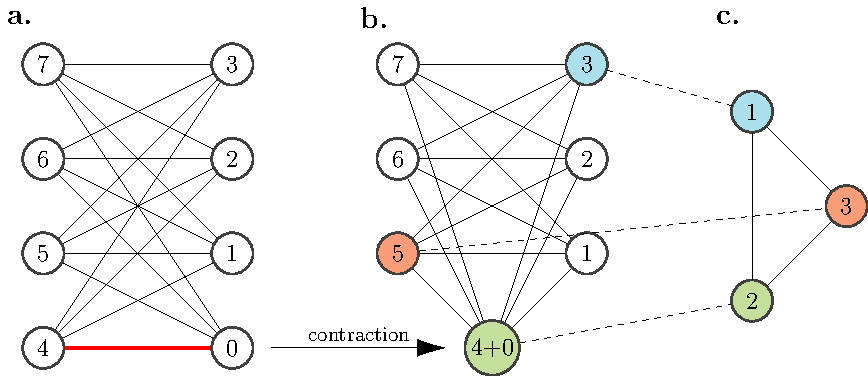
\includegraphics[width=\textwidth]{figures/minor-embedding}
    \caption{
      Example of minor embedding. Spin--glasses defined on the graph $G$
      (\textbf{c.}) cannot be directly solved on an annealer with $C_1$ topology
      (\textbf{a.}). By contracting vertices 4 and 0 one obtains a new logical graph
      $C_1'$ (\textbf{b.}), which contains $G$ as a subgraph. }
    \label{fig:minor-embedding}
  \end{figure}

  Consider an annealer with $C_1$ topology and an (arbitrary) Ising spin--glass
  instance defined on a triangular graph $G$ as depicted in Fig.
  \ref{fig:minor-embedding}. No such instance is compatible with $C_1$, because
  graph $G$ is not bipartite. Combining qubits $0$ and $4$ into a single logical
  qubit yields a graph depicted in Fig. \ref{fig:minor-embedding}\textbf{b.},
  with which $G$ is compatible. If one could use an annealer with this logical
  graph, then instances defined on $G$ could be solved directly. Note that
  vertices 0 and 4 are not the only valid choice in this case. Indeed, every
  contraction of two vertices in $C_1$ would be sufficient to embed $G$.
\end{example}

As demonstrated in the example, contracting vertices in the annealer's working
graph can make it compatible with an Ising instance otherwise unsolvable by the
annealer. It only remains to explain how this new logical graph can be used
with the actual device.

The idea is to make all the physical qubits in the chain behave like a single
qubit. Since the qubits are connected, one can couple them, including a penalty
large enough that violating qubits' alignment would prohibitively increase the
energy of the solution. The next example presents this idea.

\begin{example}[Minor embedding, continued]
  Consider an Ising spin--glass instance with Hamiltonian:

  \begin{equation}
    H(s_1, s_2, s_3) = s_1 + s_2 + s_3 - s_1s_2 - s_2s_3
  \end{equation}
  with an unique optimal solution $\mathbf{s} = (-1, -1, -1)$. Suppose we want to
  solve it on annealer with $C_1$ topology, using the minor embedding presented
  in Example \ref{ex:minor-embedding}. The problem submitted to the annealer will
  have the following Hamiltonian:
  \begin{equation}
    H'(z_0, z_3, z_4, z_5) = \underbrace{z_3 + z_5}_{s_1 + s_3} + \underbrace{0.5(z_0 + z_4)}_{s_2} - \underbrace{z_3z_4}_{s_2s_1} - \underbrace{z_0z_5}_{s_2s_3} + \underbrace{P(z_0, z_4)}_{\text{penalty}},
    \label{eq:embeddedexample}
  \end{equation}
  where $z_i$ is a spin variable associated to $i$-th qubit and $P(z_0, z_4)$ is
  a \emph{penalty term} for chain comprising qubits 0 and 4. The penalty is of
  the form
  \begin{equation}
    P(z_0, z_4) = -\alpha z_0z_4
  \end{equation}
  where $alpha$ is a positive constant. Let us examine all possible
  configurations of $(z_0, z_3, z_4, z_5)$ and observe how the penalty term
  influences their energy:
  \begin{table}[h]
    \centering
    \begin{tabular}{|c|c|c|c|}
      \hline
      \rowcolor{theader} \multicolumn{2}{|c|}{feasible solutions} & \multicolumn{2}{c|}{infeasible solutions}                                          \\
      \hline
      \rowcolor{tsubheader} $z_0, z_3, z_4, z_5$                  & energy                                    & $z_0, z_3, z_4, z_5$ & energy          \\
      \hline
      -1, -1,-1, -1                                               & $-5.0 -\alpha$                            & 1, 1,1, -1           & $1.0 + \alpha$  \\
      -1, 1,1, -1                                                 & $-2.0 -\alpha$                            & 1, -1,1, -1          & $1.0 + \alpha$  \\
      -1, -1,1, -1                                                & $-2.0 -\alpha$                            & -1, -1,-1, 1         & $-1.0 + \alpha$ \\
      1, 1,-1, 1                                                  & $2.0 -\alpha$                             & 1, 1,-1, -1          & $2.0 + \alpha$  \\
      1, -1,-1, 1                                                 & $-2.0 -\alpha$                            & 1, -1,-1, -1         & $-2.0 + \alpha$ \\
      -1, 1,-1, -1                                                & $-1.0 -\alpha$                            & -1, -1,1, 1          & $2.0 + \alpha$  \\
      1, -1,1, 1                                                  & $1.0 -\alpha$                             & -1, 1,1, 1           & $2.0 + \alpha$  \\
      1, 1,1, 1                                                   & $1.0  -\alpha$                            & -1, 1,-1, 1          & $3.0 + \alpha$  \\
      \hline
    \end{tabular}
    \caption{All possible configurations for the instance from the equation
      \eqref{eq:embeddedexample}.} \label{tab:embedded}
  \end{table}

  If $\alpha$ is large enough, e.g. $\alpha=2$, all feasible solutions (left part
  of the table) have energy lower than any solution in which qubits $z_0$ and
  $z_4$ are misaligned (right part of the table), which increases a chance of
  sampling them on a physical device. On the other hand, if $\alpha=1$, the
  feasible solution $(1,1,1,1)$ has higher energy than the infeasible solution
  $(1, -1, -1, -1)$.
\end{example}

As demonstrated in the example above, when performing minor embedding it is
important to correctly choose the chain strengths. Typically, it is not
possible to choose a correct $\alpha$ with certainty. In practice, one
typically tries different chain strengths and tests how well they perform for
the given problem.

Since the annealers are inherently heuristic devices, even with carefully
chosen chain strength one might obtain solutions that cannot be decoded into
feasible solutions to the original problem because the qubits forming chains
are misaligned. This situation is known as a \emph{chain break}, and there are
two most commonly used strategies for dealing with it:

\begin{itemize}
  \item discarding the incorrect samples. This is the simplest method, but it reduces
    the total number of samples. Hence, the experiments needing some fixed number
    of samples have to adapt and e.g. sample from the annealer multiple times until
    the desired number of feasible samples is collected.
  \item \emph{majority voting}: whenever the chain of qubits is misaligned, choose the most common value
    among the chain and use it as a value of the logical qubit. In case of a tie, choose
    -1 or 1 with equal probability.
\end{itemize}

Having presented all the necessary information about quantum annealers, we can
conclude this section with a discussion on how quantum annealing differs from
the classical model of computation.

\subsection{Comparison to the classical model of computation}
It is clear that quantum annealing is different from classical computations.
One of the most obvious differences is the computational model. On classical
computers, one essentially writes programs as a series of instructions to be
executed by the CPU. On typical machines, the CPU is capable of performing
arithmetic operations, computing values of some special functions, managing
execution flow, controlling I/O and much more. In comparison, chips in quantum
annealers are capable of executing a single operation: annealing a given
optimization problem. Therefore, programming these devices boils down to
defining an optimization problem and tuning the annealing parameters.

Another difference between classical computers and quantum annealers is the
lack of working memory in the former. Classical computers use working memory
(typically in the form of RAM) to store machine code and data. However, quantum
annealers do not need to store neither code nor data, and hence they do not
feature an analogous component. Similarly, quantum annealers, being purely
computationally oriented devices, do not have mass storage.

A slightly less obvious difference between classical computers and quantum
annealers is their model of parallelism. Classical computers are capable of
running several threads of execution at the same time. However, every
non-trivial classical algorithm involving parallelism must necessarily also
include a serial part which limits speedup gained for introducing more
execution units (CPU cores or CPUs). In contrast, quantum annealers are capable
of annealing multiple qubits at the same time, which makes their operation
inherently parallel.

\section{Nvidia CUDA}

Quantum annealing, introduced in the previous section, is a heuristic process.
Like many heuristic algorithms, it cannot certify that the solution it found is
optimal. One way to assess the performance of such algorithms is to compare
their results with known low-energy spectra of some test instances. Another
viable approach is to compute the exact low energy spectra of some test
instances, which in turn requires an exact solver. In particular, one might
perform an exhaustive search over all possible states and extract only the
selected number of the ones with the lowest energy, the approach also known as
the brute-force approach. In chapter \ref{chapter:bruteforce} we demonstrate a
massively parallel implementation of the brute-force algorithm using Nvidia
CUDA, but before we do this, in this section we will introduce the basic
principles of using CUDA-enabled graphic processing units.

\subsection{Brief history of Graphics Processing Units}
The history of specialized hardware for manipulating graphics ranges as far as
the 1970s \cite{framebuffer}. Initially, these devices, which later became
known as Graphics Processing Units (GPUs), offered limited functionalities.
Increasing demand for performance in the gaming industry and professional
graphics processing drove the evolution of GPUs, which eventually became highly
sophisticated devices supporting advanced 2D and 3D image manipulation.
Performing such arithmetically intensive operations requires enormous
computational power, and it was only a matter of time until it was realized
that the power of these devices could be harnessed for the general purpose
computations (so-called GPGPU - General Purpose computing on GPU).

The early forms of GPGPU required framing of computational problems in terms of
operations performed on graphical primitives, as this was the only way for
using specialized API of GPUs \cite{earlygpgpu,fastmatrixmultiplies}. This
changed with the development of devices, toolkits and frameworks that supported
operations needed for the general-purpose computations out of the box. Notable
examples of such computational frameworks include Nvidia CUDA \cite{CUDAguide,
  CUDAvsOpenCL, CUDAExperience} (released in 2007), ATI/AMD FireStream
\cite{firestream1,firestream2} (2006) and ROCm \cite{ROCm1,ROCm2,ROCm3} (2016)
or OpenCL \cite{CUDAvsOpenCL} (2009). The research presented in this thesis was
conducted using Nvidia CUDA-capable devices, which is why in the rest of this
chapter we focus solely on CUDA framework.

\subsection{Differences between CPU and GPU}
The principles behind the operation of CUDA-enabled GPUs are fundamentally
different from the ones governing the execution of a program on traditional
CPU-only architecture. In current x86--based computers, the CPU runs a given
sequence of instructions (so-called thread of execution) using one of its
cores. Such a processor is the ''brain'' of a computer, and it can perform a
wide variety of tasks ranging from arithmetic operations, through accessing the
system's RAM, to performing IO operations and controlling other components of
the system. Typical CPUs are optimized for sequential execution, and as such
are usually equipped with moderate (as compared to the GPUs) number of
high-performance cores.

On the other hand, GPUs are more specialized. They are well suited for
performing numerous arithmetic operations and accessing memory in parallel.
They typically have more cores than a traditional CPU (with even modern
commodity GPUs boasting thousands of them). Although those cores are less
performant than their CPU counterparts and support a much narrower set of
operations, their large number combined with fast memory access gives modern
GPUs an advantage over CPUs in multiple areas.

\subsection{Processing flow on CUDA}
Considering the architectural differences between CPUs and GPUs, it is hardly
surprising that both of these types of devices are programmed quite
differently. The first major difference is that GPUs cannot operate on their
own and are themselves controlled by the CPU. This is why CUDA is a type of
\emph{heterogenous} architecture as opposed to CPU-only \emph{homogenous}
architecture. The processing flow on CUDA is summarized in Figure
\ref{fig:cuda_flow}.

\begin{figure}[ht]
  \centering
  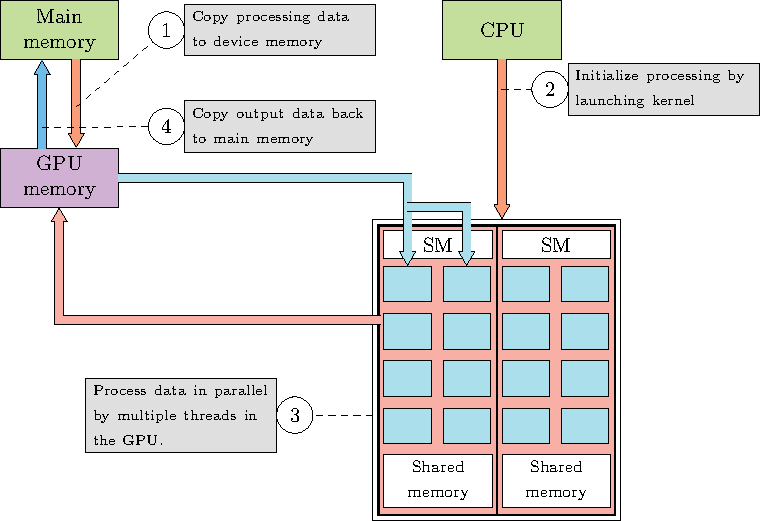
\includegraphics[width=\textwidth]{figures/cuda_workflow}
  \caption{Processing flow on CUDA. The CPU sends input data to the GPU memory and
    launches the computational kernel. The kernel's code is executed, in parallel,
    using multiple threads on the GPU. Once the execution is done, results are
    copied from the GPU memory to the system's RAM.} \label{fig:cuda_flow}
\end{figure}

Programs run on GPU are organized in \emph{kernels}. For the most part, kernels
might be viewed as functions or subroutines (which is indeed how they are
implemented) that don't have a return value. On a CPU, such a function would be
executed by some core as a part of a thread. In CUDA however, the very same
kernel is executed by multiple threads. Executing a kernel requires specifying
a \emph{grid} that will be used for running it. A grid can be 1, 2-- or
3--dimensional and is itself divided into blocks. Each block is in turn also
organized in 1, 2--, or 3-dimensional structure of threads (the same for every
block in the grid). A schematic view of a two-dimensional grid is presented in
Fig. \ref{fig:cuda_grid}.

As already mentioned, each thread in the grid executes \emph{precisely the
  same} kernel with \emph{precisely the same} parameters. It might therefore seem
surprising that, nevertheless, they can access different parts of memory or
otherwise handle a different part of the computational task. This is possible
because each thread is identified by its indices in both the grid and the
block. Those indices can be used e.g. for computing offsets in arrays that are
being processed. A more sophisticated use of thread and block indices will be
exemplified in chapter \ref{chapter:bruteforce}.

\begin{figure}[ht]
  \centering
  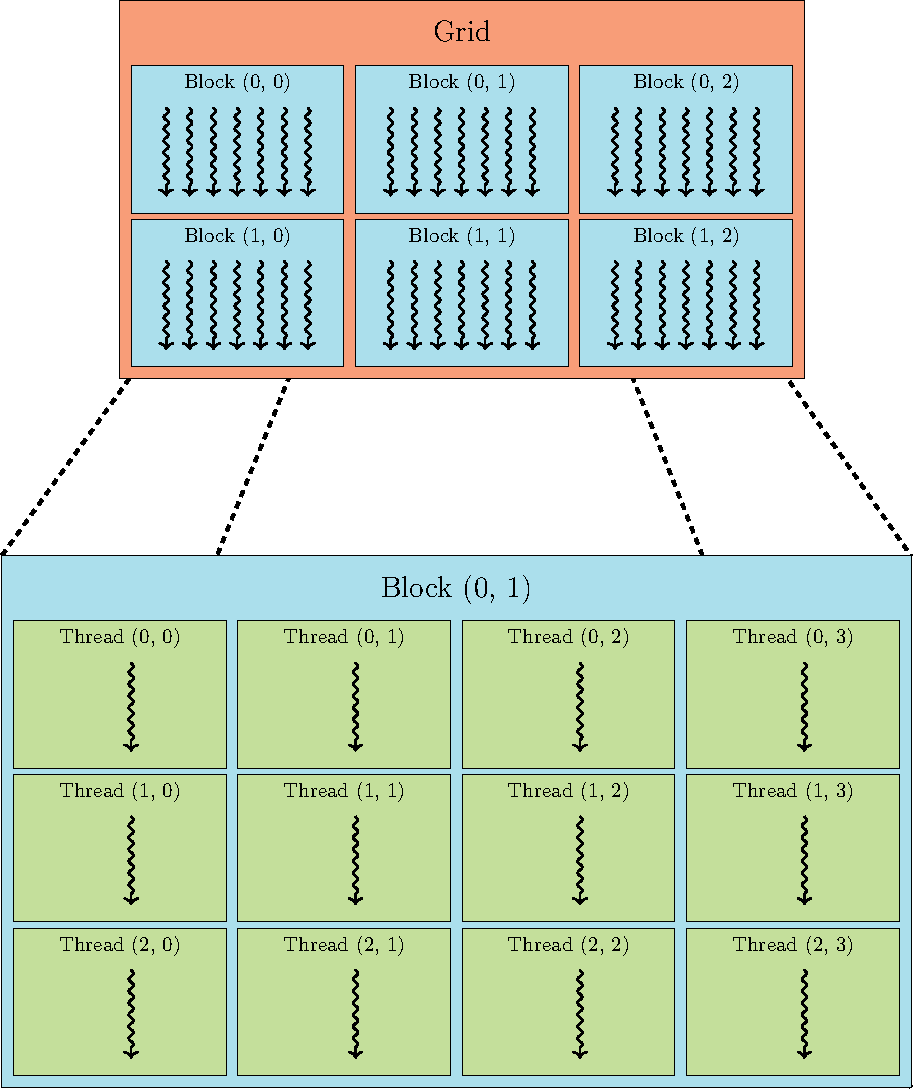
\includegraphics[width=0.9\textwidth]{figures/cuda_grid}
  \caption{A schematic view of an example two-dimensional CUDA grid. Presented here is a 2
    $\times$ 3 grid of 3 $\times$ 4 blocks.} \label{fig:cuda_grid}
\end{figure}

\subsection{SIMT architecture}
CUDA-enabled GPUs employ an architecture called SIMT (Single Instruction,
Multiple Threads)\footnote{One can contrast SIMT architecture used by CUDA with
  SIMD instructions (Single Instruction, Multiple Data) available on modern
  CPUs.}. As implied by the name, in SIMT architecture, multiple threads execute
the same instruction. Threads are executed in blocks by computational units
called Streaming Multiprocessors (SMs), and blocks are distributed to
multiprocessors on kernel launch. When a block is distributed to SM, it is
further partitioned into \emph{warps}, groups of 32 threads each. All threads
in a warp are scheduled for execution together. Nevertheless, each of them has
a separate program counter and thus their execution flow can diverge. At any
given time, a thread in a warp can be either active (executing \emph{the same}
instruction as the rest of the active threads in a warp) or inactive (not
executing any instruction at all). A thread may be inactive because its
execution diverged from the rest of the warp or because it terminated earlier.
It is interesting to note that starting from the Volta architecture, threads
can be scheduled on a finer level of granularity, allowing them to diverge and
reconverge on the sub-warp level. Each multiprocessor manages a set of 32-bit
registers and a parallel data cache, called \emph{shared memory}, distributed
among the thread blocks. Since those resources are limited, the number of warps
that can run in parallel on any SM is heavily dependent on the resource usage
of the kernel being executed.

\subsection{Memory hierarchy}

On CUDA-enabled devices, threads can access several memory types during kernel
execution, including global memory, local memory, constant and texture memory
and shared memory \cite{CUDAguide}. Physically, those different memory types
can be divided into device memory (global memory, local memory, constant
memory) and on-chip memory (shared memory). SM's on-chip memory also serves as
the L1 cache.

Global memory is a device memory available to all threads. All accesses to
global memory are serviced in 32-, 64-, or 128- bytes memory transactions.
Accesses made from a single warp are coalesced into as many such transactions
as necessary, depending on the device's architecture and access pattern. Reads
and writes targeting global memory are always cached in L2 and (depending on
configuration, compute capability and access pattern) may also be cached in L1
cache.

Local memory in CUDA is only a logical concept. Physically, it resides in the
off-chip memory just like global memory and thus offers the same bandwidth and
latency. Just like global memory, it is always cached in L2 cache. This type of
memory is never used directly by the programmer. Instead, the compiler might
decide to use it for local variables of a thread in case there is not enough
register (so-called \emph{register spilling}) or for dynamically indexed local
arrays. Local memory is arranged in such a way, that accesses are always fully
coalesced as long as all threads access the same relative address (e.g. the
same local variable, the same position of a local array etc.).

Constant and texture memory are two types of read-only
memory\footnote{Read-only here means ``Not writeable from inside the kernel''.}
residing in global memory. Accesses to constant memory are cached in constant
cache and serialized. Therefore, each request is split into as many
transactions as there are different memory addresses in the original request.
Texture memory is cached in the texture cache, which is optimized for accessing
spatial data. Hence, the best performance is achieved if threads in a warp read
or write to the addresses that are placed closely on 2D tiles.

Threads can cooperate and share data through the use of the on-chip
\emph{shared memory}. The amount of allocated shared memory is directly
controlled by the programmer either on the kernel definition level or during
its launch. Shared memory is organized in banks that can be accessed
simultaneously, and the best performance is achieved if each thread in a warp
accesses memory in a different bank. Otherwise, a \emph{bank conflict occurs},
and the request is split into as few conflict-free requests as possible.

\subsection{Programming environment}
CUDA devices can be programmed directly using either C/C++ or Fortran. For both
languages a Nvidia compiler is required to compile the CUDA program, as CUDA
extends C/C++ and Fortran languages with a syntax for defining and launching
kernels. The C/C++ CUDA code can be compiled using Nvidia's \texttt{nvcc}
compiler, shipped out of the box with the CUDA toolkit. For CUDA Fortran code,
the Nvidia High-Performance Computing (HPC) suite contains \texttt{nvfortran}
compiler\footnote{The \texttt{nvfortran} compiler was previously a third--party
  program called \texttt{pgfortran}, developed by PGI \cite{PGI}}. Giving a
comprehensive walkthrough of using either C/C++ or Fortran with CUDA is well
beyond the scope of this thesis, but for the sake of completeness, below we
present a short example of the CUDA C/C++ and CUDA Fortran code.

\begin{example}[Implementing parallel vector addition with CUDA]
  Listings \ref{lst:cuda_fortran} and \ref{lst:cuda_c} below present an example
  implementation of a parallel vector addition using CUDA. The \texttt{addVec}
  defined with \texttt{global} attribute is a kernel and accepts two input
  vectors \texttt{x}, \texttt{y} (in the form of arrays) and their length
  \texttt{n}. Since CUDA kernels cannot return a value, both versions of the code
  accept an additional argument \texttt{res} designating where the result will be
  stored. The \texttt{addVec} kernel can be launched on any one--dimensional grid
  of one--dimensional blocks. Hence, some threads may need to handle more than
  one position in the input arrays. The pattern presented here, where $i$--th
  thread handles positions $i$, $i+N$, $i+2N$, $\ldots$ with $N$ equal total
  number of blocks is called a \emph{grid-stride loop} and is illustrated in Fig.
  \ref{fig:strided-loop}.

  There are several differences between the two code examples stemming from the
  languages used. In CUDA Fortran we can copy data from the host to the GPU using
  array assignment. On the other hand, the equivalent code in C++ requires
  manually calling \texttt{cudaMemcpy} function. Similarly, the GPU arrays in C++
  are declared as pointers, for which the memory has to be manually allocated and
  later deallocated using the combination of \texttt{cudaMalloc} and
  \texttt{cudaFree}. Lastly, C/C++ uses zero-based indexing, whereas Fortran uses
  one-based indexing. This affects how the thread id, stored in \texttt{tid}
  variable, is computed.

  \begin{listing}
    \inputminted{fortran}{code/cuda_fortran.cuf}
    \caption{Example code in CUDA Fortran implementing parallel addition of vectors on GPU.}
    \label{lst:cuda_fortran}
  \end{listing}

  \begin{listing}
    \inputminted[fontsize=\footnotesize]{cuda}{code/cuda_c.cu}
    \caption{Example code in CUDA C/C++ implementing parallel addition of vectors on GPU.}
    \label{lst:cuda_c}
  \end{listing}

  \begin{figure}
    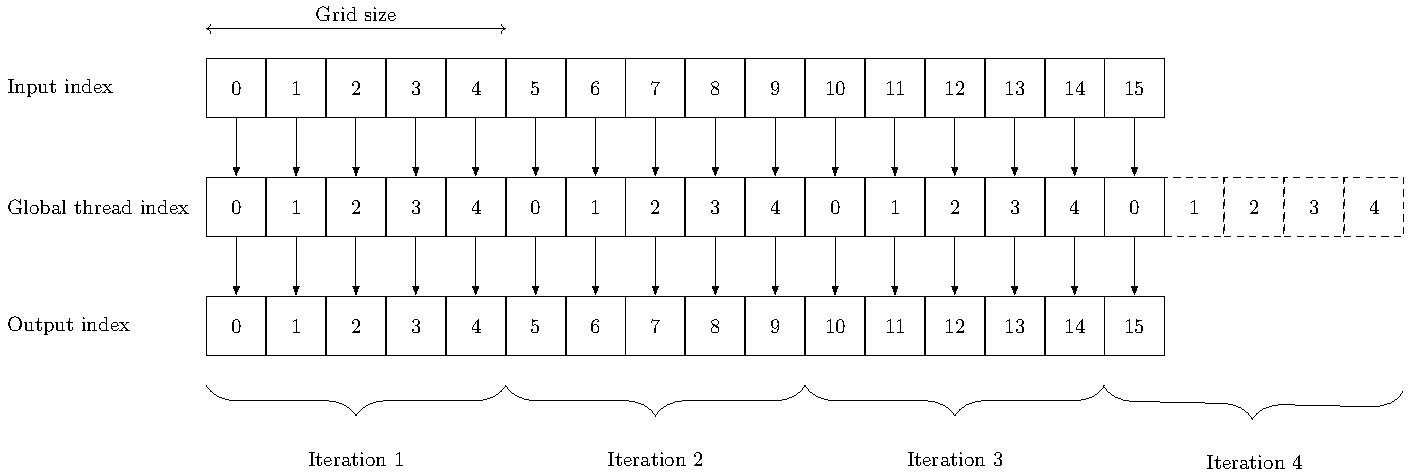
\includegraphics[width=\textwidth]{figures/gpu_scheduling}
    \caption{A schematic representation of a GPU kernel transforming an input array into an
      output array of the same size using a grid-stride loop pattern. Here, both
      arrays are of size $k=16$ and the hypothetical grid comprises $l=5$ threads
      (the exact grid configuration is irrelevant). During the first iteration, the
      $i$-th thread accesses $i$-th input element, transforms it and stores the new
      value in $i$-th element of the output array. In subsequent iterations, each
      thread advances the index it processes by the stride equal to the total grid
      size. Observe that for the last iteration only the first thread needs to do
      processing and remaining 4 threads, marked with dashed line, remain inactive. }
    \label{fig:strided-loop}
  \end{figure}

\end{example}

\subsection{Software ecosystem}
Along with the \texttt{nvcc} compiler, the CUDA toolkit contains several, more
specialized libraries. Among others, those include:
\begin{itemize}
  \item cuBLAS \cite{cublas} -- CUDA Basic Linear Algebra Subroutines library,
  \item cuFFT \cite{cufft} -- CUDA Fast Fourier Transform library,
  \item cuRAND \cite{curand} -- CUDA Random Number Generation library,
  \item cuSPARSE \cite{cusparse} -- CUDA library for manipulating sparse matrices,
  \item thrust \cite{thrust} -- parallel algorithms library. Thrust also
    provides parallel implementations of its algorithms that can be run on
    traditional CPU, making it usable even without CUDA.
\end{itemize}
For some high-level languages, there exist third-party libraries enabling the
usage of CUDA. For Python, one could mention e.g. \texttt{PyCUDA}
\cite{pycuda}, \texttt{CuPy} \cite{cupy} or recently introduced
\texttt{setuptools\_cuda} \cite{setuptoolscuda} created by the author of this
thesis. In Julia, integration with CUDA can be achieved with \texttt{CUDA.jl}
\cite{CUDAjl} package.

%%% Local Variables:
%%% mode: latex
%%% TeX-master: "../main"
%%% End:
